%% symbol library for TikZ track schematics
%
% Copyright 2018,2019,2020 Martin Scheidt (ISC license)

% Permission to use, copy, modify, and/or distribute this file for any purpose with or without fee is hereby granted, provided that the above copyright notice and this permission notice appear in all copies.

\documentclass[
  paper=a4,
  % version=3.25,
  pagesize=pdftex,
  twoside=false,
  toc=listof,
  BCOR=0pt,
  DIV=15,
]{scrartcl}

\usepackage{doc}

%%%%%% AUTHORS list %%%%%%%%%%

%\newcommand{\initials}{fullname}
\newcommand{\MS}{Martin Scheidt}

%%%%%%%%%%%%%%%%%%%%%%%%%%%%%%

% -------[ PDF Informations ]---------
\hypersetup{%
  pdftitle={tikz/trackschematic},
  pdfsubject={A tikz toolbox for track schematics},
  pdfauthor={Martin Scheidt},
  pdfkeywords={latex, tikz, library, railway, track, layout}
}

\begin{document}

\title{\tikz\node[scale=1.2]{\color{gray}\Huge\sffamily \{\textcolor{black}{Ti\textcolor{orange}{\emph{k}}Z}-\textcolor{blue}{trackschematic}\}};}
\subtitle{A Ti\emph{k}Z library for track schematics}
\author{\vhListAllAuthorsLong}
\date{Version \vhCurrentVersion~ from \vhCurrentDate}

\maketitle

\begin{multicols}{2}
  \tableofcontents
\end{multicols}
\cleardoublepage

\section{Introduction}\label{sec:intro}

  \subsection[About]{About tikz-trackschematic}

    The Ti\emph{k}Z-\emph{trackschematic} library is a toolbox of symbols geared primarily towards creating track schematic for either research or educational purposes.
    It provides a Ti\emph{k}Z frontend to some of the symbols which maybe needed to describe situations and layouts in railway operation.
    The library is divided into four sublibraries:
    \begin{itemize*}[label={}]
      \item \texttt{topology},
      \item \texttt{trafficcontrol},
      \item \texttt{vehicles},
      \item \texttt{constructions}, and
      \item \texttt{messures}.
    \end{itemize*}

  \subsection{Acknowledgement}

    This project has received funding from the European Union’s Horizon 2020 research and innovation programme under grant agreement No. 826347.

  \subsection{Requirements}\label{sec:require}

    The library uses Ti\emph{k}Z and it is based the following packages:
    \begin{itemize*}[label={}]
      \item \texttt{tikz},
      \item \texttt{lmodern},
      \item \texttt{xcolor}, and
      \item \texttt{etoolbox}.
    \end{itemize*}
    Further more it uses the following Ti\emph{k}Z libraries:
    \begin{itemize*}[label={}]
      \item \texttt{calc},
      \item \texttt{intersections},
      \item \texttt{patterns}, and
      \item \texttt{arrows.meta}.
    \end{itemize*}


  \subsection{License}

    Copyright (c) 2018 - 2020, \MS.
    Permission to use, copy, modify, and/or distribute this file for any purpose with or without fee is hereby granted, provided that the above copyright notice and this permission notice appear in all copies (\href{https://www.tldrlegal.com/l/isc}{ISC license}).

  \subsection{Alternatives}

    Apart from this library, there is also a \href{https://tu-dresden.de/bu/verkehr/ibv/vst/die-professur/mitarb/ulrich-maschek/signalschablone}{Signalschablone} with german (Deutsche Bahn) symbols for MS Visio.


% \newpage
\section{Usage}\label{sec:use}
  \subsection{A complete minimal example}

    The command \texttt{\textbackslash usetikzlibrary\{trackschematic\}} will load the library; place it somewhere in your preamble.
    Here is a complete working minimal example which will produce a single PDF file with the figure on the right:\\
    \begin{minipage}[c]{0.51\textwidth}
      \centering
      \begin{lstlisting}[gobble=8]
        \documentclass[tikz]{standalone}

        % loading the library
        \usetikzlibrary{trackschematic}

        \begin{document}
          \begin{tikzpicture}

            % draw a track
            \maintrack  (0,0) -- (6,0);

            % place a train on the track
            \train[forward] at (5,0) label ();

          \end{tikzpicture}
        \end{document}
      \end{lstlisting}
    \end{minipage}
    \hfil
    \begin{minipage}[c]{0.45\textwidth}
      \centering
      \begin{tikzpicture}
        \path (-0.2,-1.45) rectangle (6.2,1.45);
        \coordinate (A) at (0,0);
        \coordinate (T) at (5,0);
        \coordinate (B) at (6,0);
        \maintrack  (A) -- (B);
        \train[forward] at (T) label ();
      \end{tikzpicture}
    \end{minipage}

  \subsection{Placement}\label{sec:placement}

    To place symbols in a track schematic, they need to placed and oriented correctly.
    The placement ist done through the given Ti\emph{k}Z coordinate.
    There are a few assumaptions made about the placement:
    \begin{enumerate}
      \item Parallel tracks are drawn at a distance of 1 cm (which is the base unit of Ti\emph{k}Z).
      \item Tracks are only drawn at an angle of $n \cdot 45^{\circ}$.
    \end{enumerate}

  \subsection{Orientation system}\label{sec:orientationsystem}

    The orientation is controlled via given Ti\emph{k}Z options or pgfkey.
    The orientation options/pgfkeys are named in relation to orientation-based coordinates, which inhibate thier meaning from reading left to right beeing \texttt{forward} and relate \texttt{left}/\texttt{right} to that movement.
    \begin{center}
      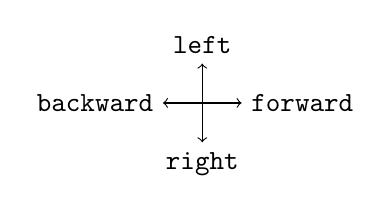
\begin{tikzpicture}[font=\ttfamily]
        \draw[<->] (-0.5,0) node[left] {backward} -- (0.5,0) node[right] {forward};
        \draw[<->] (0,-0.5) node[below] {right} -- (0,0.5) node[above] {left};
      \end{tikzpicture}
    \end{center}

    The main option/pgfkey is the \texttt{face} option to control in which direction an object will face.
    The key can take one of the following two values:
    \begin{itemize*}[label={}]
      \item \texttt{forward}, and
      \item \texttt{backward}.
    \end{itemize*}
    \begin{minipage}[c]{0.68\textwidth}
    \begin{lstlisting}[gobble=6]

      \train[face=forward ] at (coordinate) label ();

    \end{lstlisting}
    \end{minipage}
    \hfil
    \begin{minipage}[c]{0.30\textwidth}
      \tikz{\train[face=forward] at (5,0) label ();}
    \end{minipage}
    \begin{minipage}[c]{0.68\textwidth}
    \begin{lstlisting}[gobble=6]

      \train[face=backward] at (coordinate) label ();

    \end{lstlisting}
    \end{minipage}
    \hfil
    \begin{minipage}[c]{0.30\textwidth}
      \tikz{\train[face=backward] at (1,0) label ();}
    \end{minipage}
    As a shortcut you may also just give the option \texttt{forward} or \texttt{backward} without the \texttt{face=} in front of it.

    If you have objects which branch either to the left or the right you have to give the \texttt{branch} option which takes one of the following two values:
    \begin{itemize*}[label={}]
      \item \texttt{left}, and
      \item \texttt{right}.
    \end{itemize*}\\
    \begin{minipage}[c]{0.68\textwidth}
    \begin{lstlisting}[gobble=6]

      \turnout[forward ,branch=left ] at (coordinate) label ();

    \end{lstlisting}
    \end{minipage}
    \hfil
    \begin{minipage}[c]{0.30\textwidth}
      \tikz{\maintrack (0,0)--(4,0);\maintrack (2,0)--++(0.5,0.5);\turnout[forward,branch=left] at (2,0) label ();}
    \end{minipage}
    \begin{minipage}[c]{0.68\textwidth}
    \begin{lstlisting}[gobble=6]

      \turnout[forward ,branch=right] at (coordinate) label ();

    \end{lstlisting}
    \end{minipage}
    \hfil
    \begin{minipage}[c]{0.30\textwidth}
      \tikz{\maintrack (0,0)--(4,0);\maintrack (2,0)--++(0.5,-0.5);\turnout[forward,branch=right] at (2,0) label ();}
    \end{minipage}
    \begin{minipage}[c]{0.68\textwidth}
    \begin{lstlisting}[gobble=6]

      \turnout[backward,branch=left ] at (coordinate) label ();

    \end{lstlisting}
    \end{minipage}
    \hfil
    \begin{minipage}[c]{0.30\textwidth}
      \tikz{\maintrack (0,0)--(4,0);\maintrack (2,0)--++(-0.5,0.5);\turnout[backward,branch=left] at (2,0) label ();}
    \end{minipage}
    \begin{minipage}[c]{0.68\textwidth}
    \begin{lstlisting}[gobble=6]

      \turnout[backward,branch=right] at (coordinate) label ();

    \end{lstlisting}
    \end{minipage}
    \hfil
    \begin{minipage}[c]{0.30\textwidth}
      \tikz{\maintrack (0,0)--(4,0);\maintrack (2,0)--++(-0.5,-0.5);\turnout[backward,branch=right] at (2,0) label ();}
    \end{minipage}
    There is no shortcut and the key \texttt{branch=} must be given contrary to the key \texttt{face=}.

  \subsection{Left- and right-hand traffic}\label{sec:traffic}

    The traffic practice to divide bidirectional traffic has impact mostly on traffic control.
    The default traffic practice for this library ist right-hand traffic.
    You can change it either globally or locally with the key \texttt{traffic practice=left}.
    There is also the alias \texttt{position} for single local entries.
    \begin{minipage}[c]{0.65\textwidth}
      \begin{lstlisting}[gobble=8]
        \documentclass[tikz]{standalone}

        % load the library
        \usetikzlibrary{trackschematic}

        \begin{document}
          \begin{tikzpicture}
            % set the traffic practice
            \tikzset{traffic practice=left}

            \maintrack  (0,1) -- (5,1);
            \maintrack  (0,0) -- (5,0);
            \routesignal[forward]                at (2,1) label (left);
            \routesignal[forward,position=right] at (2,0) label (right);
          \end{tikzpicture}
        \end{document}
      \end{lstlisting}
    \end{minipage}
    \hfil
    \begin{minipage}[c]{0.34\textwidth}
      \begin{tikzpicture}
        \tikzset{traffic practice=left}
        \path (-0.2,-1.6) rectangle (5.2,2.6);
        \coordinate (A1) at (0,1);
        \coordinate (S1) at (2,1);
        \coordinate (B1) at (5,1);
        \maintrack  (A1) -- ( B1);
        \coordinate (A2) at (0,0);
        \coordinate (S2) at (2,0);
        \coordinate (B2) at (5,0);
        \maintrack  (A2) -- ( B2);
        \routesignal[forward] at (S1) label (left);
        \routesignal[forward,position=right] at (S2) label (right);
      \end{tikzpicture}
    \end{minipage}

  \subsection{Colors: background and foreground}\label{sec:colors}

    The two main colors \texttt{white} and \texttt{black} are set for the \texttt{background} and \texttt{foreground} keys by default.
    If you want to change them, provide a new value for the keys.
    For example like this:\\
    \begin{minipage}[c]{0.65\textwidth}
      \begin{lstlisting}[gobble=8]
        \documentclass[tikz]{standalone}

        % load the library
        \usetikzlibrary{trackschematic}

        \begin{document}
          \begin{tikzpicture}
            % set the colors
            \tikzset{background=lightgray,foreground=violet}

            \maintrack  (0,0) -- (6,0);
            \train[forward] at (5,0) label (grey train);
          \end{tikzpicture}
        \end{document}
      \end{lstlisting}
    \end{minipage}
    \hfil
    \begin{minipage}[c]{0.34\textwidth}
      \begin{tikzpicture}
        \tikzset{background=lightgray,foreground=violet}
        \path (-0.2,-1.6) rectangle (5.2,1.6);
        \coordinate (A) at (0  ,0);
        \coordinate (T) at (4.5,0);
        \coordinate (B) at (5  ,0);
        \maintrack  (A) -- (B);
        \train[forward] at (T) label (grey train);
      \end{tikzpicture}
    \end{minipage}


\section{Provided Symbols and their commands}

  Each sublibrary provides different symbols. The following section will go through each symbol their command and options.
  % for aperance see the snippet document

  \subsection{Topology}
    
    \subsubsection{Tracks}\label{sec:track}

      Drawing a track follows the same pricipal as drawing a line in Ti\emph{k}Z.
      There are two generell optionss of track with different commands:
      \begin{itemize*}[label={}]
        \item \texttt{main tracks}, and
        \item \texttt{secondary tracks}.
      \end{itemize*}

      \symboldescription{Main track}
        \symbol{main_track.tikz}
        \begin{lstlisting}[gobble=10]
          \maintrack (coord1) -- (coord2);
          \maintrack (coord1) -- (coord2) -- (coord3) -- etc.;
        \end{lstlisting}
        No \texttt{options} available.\\
        This command is equivalent to:
        \begin{lstlisting}[gobble=10]
          \path[draw=foreground,line width=2pt] (coord1) -- (coord2);
        \end{lstlisting}
        Beware of the placement assumption by the library (see Section \ref{sec:placement}).


      \symboldescription{Secondary track}
        \symbol{secondary_track.tikz}
        \begin{lstlisting}[gobble=10]
          \secondarytrack (coord1) -- (coord2);
          \secondarytrack (coord1) -- (coord2) -- (coord3) -- etc.;
        \end{lstlisting}
        For the secondary track you may also use the following alias:
        \begin{lstlisting}[gobble=10]
          \sidetrack (coord1) -- (coord2);
        \end{lstlisting}
        No \texttt{options} available.\\
        The command is equivalent to:
        \begin{lstlisting}[gobble=10]
          \path[draw=foreground,line width=0.7pt] (coord1) -- (coord2);
        \end{lstlisting}
        Beware of the placement assumption by the library (see Section \ref{sec:placement}).

      \symboldescription{Track number or track label}
        \symbol{track_number.tikz}
        \begin{lstlisting}[gobble=10]
          \tracklabel at (coord) label (number);
        \end{lstlisting}
        No \texttt{options} available.\\
        This command is equivalent to:
        \begin{lstlisting}[gobble=10]
          \node[fill=background,text=foreground] at (coord) {number};
        \end{lstlisting}

      \symboldescription{Buffer stops}
        \symbol{bufferstop_forward.tikz}
        \symbol{friction_bufferstop_forward.tikz}
        \begin{lstlisting}[gobble=10]
          \bufferstop[options] at (coord);
        \end{lstlisting}
        values for \texttt{options} (comma seperated):
        \begin{itemize}[label={}]
          \item \texttt{forward} or \texttt{backward} (mandatory)
          \item \texttt{friction=\textit{length unit}} (optional)
          \item \texttt{foreground=\textit{color}} (optional, default: \texttt{black})
        \end{itemize}

      \symboldescription{Track closures}
        \symbol{track_closure.tikz}
        \begin{lstlisting}[gobble=10]
          \trackclosure at (coord);
        \end{lstlisting}
        No \texttt{options} available.\\

    \subsubsection{Turnouts and similar}\label{sec:turnout}
      \symboldescription{Turnouts}
        \symbol{turnout_with_fouling_left_forward.tikz}
        \symbol{turnout_left_forward_manually.tikz}
        % \symbol{turnout_left_forward_right_position.tikz}
        \begin{lstlisting}[gobble=10]
          \turnout[options] at (coord) label (name);
        \end{lstlisting}
        values for \texttt{options} (comma seperated):
        \begin{itemize}[label={}]
          \item \texttt{forward} or \texttt{backward} (mandatory)
          \item \texttt{branch=left} or \texttt{branch=right} (mandatory)
          \item \texttt{operation=manual} (optional) % \texttt{operation=remote} (default)
          \item \texttt{fouling point} (optional)
          \item \texttt{points=left} or \texttt{points=right} (optional)
          \item \texttt{shift label=\{\textit{(label-coord)}\}} (optional, default: (0,0))
          \item \texttt{foreground=\textit{color}} (optional, default: \texttt{black})
        \end{itemize}

      \symboldescription{Diamond crossings}
        \symbol{diamond_crossing_left.tikz}
        \begin{lstlisting}[gobble=10]
          \crossing[options] at (coord) label (name);
        \end{lstlisting}
        values for \texttt{options} (comma seperated):
        \begin{itemize}[label={}]
          \item \texttt{branch=left} or \texttt{branch=right} (mandatory)
          \item \texttt{fouling point} (optional)
        \item \texttt{shift label=\{\textit{(label-coord)}\}} (optional, default: (0,0))
          \item \texttt{foreground=\textit{color}} (optional, default: \texttt{black})
        \end{itemize}

      \symboldescription{Slip switchs or slip turnouts}
        \symbol{double-slip_turnout_left.tikz}
        \begin{lstlisting}[gobble=10]
          \slipturnout[options] at (coord) label (name1)(name2);
        \end{lstlisting}
        values for \texttt{options} (comma seperated):
        \begin{itemize}[label={}]
          \item \texttt{branch=left} or \texttt{branch=right} (mandatory)
          \item \texttt{slip=double} (default), \texttt{slip=none}, \texttt{slip=left} or \texttt{slip=right} (mandatory)
          \item \texttt{operation=manual} (optional) % \texttt{operation=remote} (default)
          \item \texttt{fouling point} (optional)
          \item \texttt{forward points=left} or \texttt{forward points=right} (optional)
          \item \texttt{backward points=left} or \texttt{backward points=right} (optional)
          \item \texttt{shift label=\{\textit{(label-coord)}\}} (optional, default: (0,0))
          \item \texttt{foreground=\textit{color}} (optional, default: \texttt{black})
        \end{itemize}

      \symboldescription{Derailers}
        \symbol{derailer_left_forward.tikz}
        \begin{lstlisting}[gobble=10]
          \derailer[options] at (coord) label (name);
        \end{lstlisting}
        values for \texttt{options} (comma seperated):
        \begin{itemize}[label={}]
          \item \texttt{forward} or \texttt{backward} (mandatory)
          \item \texttt{branch=left} or \texttt{branch=right} (mandatory)
          \item \texttt{shift label=\{\textit{(label-coord)}\}} (optional, default: (0,0))
          \item \texttt{foreground=\textit{color}} (optional, default: \texttt{black})
        \end{itemize}

  \subsection{Vehicles}\label{sec:vehicles}

    \symboldescription{Parked vehicles}\label{sec:parked}
      \symbol{parked_vehicles.tikz}
      \begin{lstlisting}[gobble=8]
        \parkedvehicles[options] at (coord) label (name);
      \end{lstlisting}
      values for \texttt{options} (comma seperated):
      \begin{itemize}[label={}]
        \item \texttt{length=\textit{length unit}} (optional, default 4cm)
        \item \texttt{label at=\{\textit{(label-coord)}\}} (optional, default: \textit{center})
        \item \texttt{label align=left} or \texttt{label align=right} (optional, default: center)
        \item \texttt{foreground=\textit{color}} (optional, default: \texttt{black})
        \item \texttt{background=\textit{color}} (optional, default: \texttt{white})
      \end{itemize}
      The value for \textit{(label-coord)} is relative to \textit{(coord)}.
      An absolute \textit{(label-coord)} can be specified with the Ti\emph{k}Z \textbackslash coordinate command.

    \symboldescription{Shunting movements}\label{sec:shunting}
      % \symbol{train_shunt_mode_forward.tikz}
      \symbol{train_shunting_forward.tikz}
      \begin{lstlisting}[gobble=8]
        \shunting[options] at (coord) label (name);
      \end{lstlisting}
      values for \texttt{options} (comma seperated):
      \begin{itemize}[label={}]
        \item \texttt{movement} (optional)
        \item \texttt{forward} or \texttt{backward} (mandatory)
        \item \texttt{length=\textit{length unit}} (optional, default 4cm)
        \item \texttt{operation=manual} or \texttt{operation=automatic} (optional) % \texttt{operation=undefined} (default)
        \item \texttt{bend left at=\{\textit{(bend-coord)}\}} (optional, default: \textit{none})
        \item \texttt{bend right at=\{\textit{(bend-coord)}\}} (optional, default: \textit{none})
        \item \texttt{label at=\{\textit{(label-coord)}\}} (optional, default: \textit{center})
        \item \texttt{label align=left} or \texttt{label align=right} (optional, default: center)
        \item \texttt{foreground=\textit{color}} (optional, default: \texttt{black})
        \item \texttt{background=\textit{color}} (optional, default: \texttt{white})
      \end{itemize}
      The value for \textit{(label-coord)} and \textit{(bend-coord)} is relative to \textit{(coord)}.
      An absolute \textit{(label-coord)} or \textit{(bend-coord)} can be specified with the Ti\emph{k}Z \textbackslash coordinate command.

    \symboldescription{Train runs}\label{sec:train}
      \symbol{train_moving_fast_forward.tikz}
      \symbol{train_ghost_direction_forward.tikz}
      \begin{lstlisting}[gobble=8]
        \train[options] at (coord) label (name);
      \end{lstlisting}
      values for \texttt{options} (comma seperated):
      \begin{itemize}[label={}]
        \item \texttt{run=slow}, \texttt{run=normal} or \texttt{run=fast} (optional)
        \item \texttt{forward} or \texttt{backward} (mandatory)
        \item \texttt{length=\textit{length unit}} (optional, default 4cm)
        \item \texttt{operation=manual} or \texttt{operation=automatic} (optional) % \texttt{operation=undefined} (default)
        \item \texttt{ghost} (optional)
        \item \texttt{bend left at=\{\textit{(bend-coord)}\}} (optional, default: \textit{none})
        \item \texttt{bend right at=\{\textit{(bend-coord)}\}} (optional, default: \textit{none})
        \item \texttt{shift label=\{\textit{(label-coord)}\}} (optional, default: (0,0))
        \item \texttt{label align=left} or \texttt{label align=right} (optional, default: center)
        \item \texttt{foreground=\textit{color}} (optional, default: \texttt{black})
        \item \texttt{background=\textit{color}} (optional, default: \texttt{white})
      \end{itemize}
      The value for \textit{(label-coord)} and \textit{(bend-coord)} is relative to \textit{(coord)}.
      An absolute \textit{(label-coord)} or \textit{(bend-coord)} can be specified with the Ti\emph{k}Z \textbackslash coordinate command.

  \subsection{Traffic control}
    \subsubsection{Signals}\label{sec:signals}
      
      \symboldescription{Generic signal command}
        \begin{lstlisting}[gobble=10]
          \signal[options] at (coord) label (name);
        \end{lstlisting}
        values for \texttt{options} (comma seperated):
        \begin{itemize}[label={}]
          \item at least one of the following: 
          \begin{enumerate*}[label={}]
            \item \texttt{distant},
            \item \texttt{speed type},
            \item \texttt{block},
            \item \texttt{route},
            \item \texttt{shunt limit},
            \item \texttt{shunting} and/or
            \item \texttt{berth}
          \end{enumerate*}
          \item \texttt{forward} or \texttt{backward} (mandatory)
          \item \texttt{speed=\textit{value}} (optional)
          \item \texttt{distant speed=\textit{value}} (optional)
          \item \texttt{locked=false} (default) or \texttt{locked=true} (optional)
          \item \texttt{position=left} or \texttt{position=right} (optional, default: \textit{traffic practice})
          \item \texttt{shift label=\{\textit{(label-coord)}\}} (optional, default: (0,0))
          \item \texttt{foreground=\textit{color}} (optional, default: \texttt{black})
        \end{itemize}

      \symboldescription{Distant signal}
        \symbol{distant_signal_forward.tikz}
        \begin{lstlisting}[gobble=10]
          \distantsignal[options] at (coord) label (name);
        \end{lstlisting}
        values for \texttt{options} (comma seperated):
        \begin{itemize}[label={}]
          \item \texttt{forward} or \texttt{backward} (mandatory)
          \item \texttt{distant speed=\textit{value}} (optional)
          \item \texttt{position=left} or \texttt{position=right} (optional, default: \textit{traffic practice})
          \item \texttt{shift label=\{\textit{(label-coord)}\}} (optional, default: (0,0))
          \item \texttt{foreground=\textit{color}} (optional, default: \texttt{black})
        \end{itemize}
        This command is equivalent to:
        \begin{lstlisting}[gobble=10]
          \signal[distant,options] at (coord) label (name);
        \end{lstlisting}

      \symboldescription{Speed signal/sign}
        \symbol{speed_signal_forward.tikz}
        \begin{lstlisting}[gobble=10]
          \speedsignal[options] at (coord) label (name);
        \end{lstlisting}
        For the speed signal you may also use the following alias:
        \begin{lstlisting}[gobble=10]
          \speedsign[options] at (coord) label (name);
        \end{lstlisting}
        values for \texttt{options} (comma seperated):
        \begin{itemize}[label={}]
          \item \texttt{forward} or \texttt{backward} (mandatory)
          \item \texttt{speed=\textit{value}} (optional)
          \item \texttt{position=left} or \texttt{position=right} (optional, default: \textit{traffic practice})
          \item \texttt{shift label=\{\textit{(label-coord)}\}} (optional, default: (0,0))
          \item \texttt{foreground=\textit{color}} (optional, default: \texttt{black})
        \end{itemize}
        This command is equivalent to:
        \begin{lstlisting}[gobble=10]
          \signal[speed type,options] at (coord) label (name);
        \end{lstlisting}

      \symboldescription{Block signal}
        \symbol{block_signal_forward.tikz}
        \begin{lstlisting}[gobble=10]
          \blocksignal[options] at (coord) label (name);
        \end{lstlisting}
        values for \texttt{options} (comma seperated):
        \begin{itemize}[label={}]
          \item \texttt{forward} or \texttt{backward} (mandatory)
          \item \texttt{speed=\textit{value}} (optional)
          \item \texttt{position=left} or \texttt{position=right} (optional, default: \textit{traffic practice})
          \item \texttt{shift label=\{\textit{(label-coord)}\}} (optional, default: (0,0))
          \item \texttt{foreground=\textit{color}} (optional, default: \texttt{black})
        \end{itemize}
        This command is equivalent to:
        \begin{lstlisting}[gobble=10]
          \signal[block,options] at (coord) label (name);
        \end{lstlisting}

      \symboldescription{Route signal}
        \symbol{route_signal_forward.tikz}
        \begin{lstlisting}[gobble=10]
          \routesignal[options] at (coord) label (name);
        \end{lstlisting}
        values for \texttt{options} (comma seperated):
        \begin{itemize}[label={}]
          \item \texttt{forward} or \texttt{backward} (mandatory)
          \item \texttt{speed=\textit{value}} (optional)
          \item \texttt{locked=false} (default) or \texttt{locked=true} (optional)
          \item \texttt{position=left} or \texttt{position=right} (optional, default: \textit{traffic practice})
          \item \texttt{shift label=\{\textit{(label-coord)}\}} (optional, default: (0,0))
          \item \texttt{foreground=\textit{color}} (optional, default: \texttt{black})
        \end{itemize}
        This command is equivalent to:
        \begin{lstlisting}[gobble=10]
          \signal[route,options] at (coord) label (name);
        \end{lstlisting}

      \symboldescription{Shunting signal}
        \symbol{shunt_signal_forward.tikz}
        \begin{lstlisting}[gobble=10]
          \shuntsignal[options] at (coord) label (name);
        \end{lstlisting}
        values for \texttt{options} (comma seperated):
        \begin{itemize}[label={}]
          \item \texttt{forward} or \texttt{backward} (mandatory)
          \item \texttt{locked=false} (default) or \texttt{locked=true} (optional)
          \item \texttt{position=left} or \texttt{position=right} (optional, default: \textit{traffic practice})
          \item \texttt{shift label=\{\textit{(label-coord)}\}} (optional, default: (0,0))
          \item \texttt{foreground=\textit{color}} (optional, default: \texttt{black})
        \end{itemize}
        This command is equivalent to:
        \begin{lstlisting}[gobble=10]
          \signal[shunting,options] at (coord) label (name);
        \end{lstlisting}

      \symboldescription{Shunt limit}
        \symbol{shunt_limit_forward.tikz}
        \begin{lstlisting}[gobble=10]
          \shuntlimit[options] at (coord) label (name);
        \end{lstlisting}
        values for \texttt{options} (comma seperated):
        \begin{itemize}[label={}]
          \item \texttt{forward} or \texttt{backward} (mandatory)
          \item \texttt{position=left} or \texttt{position=right} (optional, default: \textit{traffic practice})
          \item \texttt{shift label=\{\textit{(label-coord)}\}} (optional, default: (0,0))
          \item \texttt{foreground=\textit{color}} (optional, default: \texttt{black})
        \end{itemize}
        This command is equivalent to:
        \begin{lstlisting}[gobble=10]
          \signal[shunt limit,options] at (coord) label (name);
        \end{lstlisting}

      \symboldescription{Berth signal/sign}
        \symbol{train_berth_sign_forward.tikz}
        \begin{lstlisting}[gobble=10]
          \berthsignal[options] at (coord) label (name);
        \end{lstlisting}
        For the speed signal you may also use the following alias:
        \begin{lstlisting}[gobble=10]
          \berthsign[options] at (coord) label (name);
        \end{lstlisting}
        values for \texttt{options} (comma seperated):
        \begin{itemize}[label={}]
          \item \texttt{forward} or \texttt{backward} (mandatory)
          \item \texttt{position=left} or \texttt{position=right} (optional, default: \textit{traffic practice})
          \item \texttt{shift label=\{\textit{(label-coord)}\}} (optional, default: (0,0))
          \item \texttt{foreground=\textit{color}} (optional, default: \texttt{black})
        \end{itemize}
        This command is equivalent to:
        \begin{lstlisting}[gobble=10]
          \signal[berth,options] at (coord) label (name);
        \end{lstlisting}

    \subsubsection{Clearing points}\label{sec:clearingpoints}

      \symboldescription{Generic clearing point}
        \begin{lstlisting}[gobble=10]
          \clearingpoint[options] at (coord) label (name);
        \end{lstlisting}
        values for \texttt{options} (comma seperated):
        \begin{itemize}[label={}]
          \item at least one of the following: 
          \begin{enumerate*}[label={}]
            \item \texttt{standard},
            \item \texttt{block} and/or
            \item \texttt{route}
          \end{enumerate*}
          \item \texttt{forward} (default) or \texttt{backward} (optional)
          \item \texttt{position=left} or \texttt{position=right} (optional, default: \textit{traffic practice})
          \item \texttt{shift label=\{\textit{(label-coord)}\}} (optional, default: (0,0))
          \item \texttt{foreground=\textit{color}} (optional, default: \texttt{black})
        \end{itemize}

      \symboldescription{Standard clearing point}
        \symbol{clearing_point.tikz}
        \begin{lstlisting}[gobble=10]
          \standardclearing[options] at (coord) label (name);
        \end{lstlisting}
        values for \texttt{options} (comma seperated):
        \begin{itemize}[label={}]
          \item \texttt{forward} (default) or \texttt{backward} (optional)
          \item \texttt{position=left} or \texttt{position=right} (optional, default: \textit{traffic practice})
          \item \texttt{shift label=\{\textit{(label-coord)}\}} (optional, default: (0,0))
          \item \texttt{foreground=\textit{color}} (optional, default: \texttt{black})
        \end{itemize}
        This command is equivalent to:
        \begin{lstlisting}[gobble=10]
          \clearingpoint[standard,options] at (coord) label (name);
        \end{lstlisting}

      \symboldescription{Block clearing point}
        \symbol{block_clearing_point_forward.tikz}
        \begin{lstlisting}[gobble=10]
          \blockclearing[options] at (coord) label (name);
        \end{lstlisting}
        values for \texttt{options} (comma seperated):
        \begin{itemize}[label={}]
          \item \texttt{forward} (default) or \texttt{backward} (optional)
          \item \texttt{position=left} or \texttt{position=right} (optional, default: \textit{traffic practice})
          \item \texttt{shift label=\{\textit{(label-coord)}\}} (optional, default: (0,0))
          \item \texttt{foreground=\textit{color}} (optional, default: \texttt{black})
        \end{itemize}
        This command is equivalent to:
        \begin{lstlisting}[gobble=10]
          \clearingpoint[block,options] at (coord) label (name);
        \end{lstlisting}

      \symboldescription{Route clearing point}
        \symbol{route_clearing_point_forward.tikz}
        \begin{lstlisting}[gobble=10]
          \routeclearing[options] at (coord) label (name);
        \end{lstlisting}
        values for \texttt{options} (comma seperated):
        \begin{itemize}[label={}]
          \item \texttt{forward} (default) or \texttt{backward} (optional)
          \item \texttt{position=left} or \texttt{position=right} (optional, default: \textit{traffic practice})
          \item \texttt{shift label=\{\textit{(label-coord)}\}} (optional, default: (0,0))
          \item \texttt{foreground=\textit{color}} (optional, default: \texttt{black})
        \end{itemize}
        This command is equivalent to:
        \begin{lstlisting}[gobble=10]
          \clearingpoint[route,options] at (coord) label (name);
        \end{lstlisting}

    \subsubsection{Transmitters}\label{sec:transmitters}

      \symboldescription{Generic transmitter command}
        \begin{lstlisting}[gobble=10]
          \transmitter[options] at (coord) label (name);
        \end{lstlisting}
        values for \texttt{options} (comma seperated):
        \begin{itemize}[label={}]
          \item \texttt{type=balise} or \texttt{type=loop} (mandatory)
          \item \texttt{forward}, \texttt{backward} or \texttt{bidirectional} (optional)
          \item \texttt{position=left} or \texttt{position=right} (optional, default: \textit{traffic practice})
          \item \texttt{shift label=\{\textit{(label-coord)}\}} (optional, default: (0,0))
          \item \texttt{foreground=\textit{color}} (optional, default: \texttt{black})
        \end{itemize}

      \symboldescription{Balise}
        \symbol{transmitter_right_bidirectional.tikz}
        \begin{lstlisting}[gobble=10]
          \balise[options] at (coord) label (name);
        \end{lstlisting}
        values for \texttt{options} (comma seperated):
        \begin{itemize}[label={}]
          \item \texttt{forward}, \texttt{backward} or \texttt{bidirectional} (optional)
          \item \texttt{position=left} or \texttt{position=right} (optional, default: \textit{traffic practice})
          \item \texttt{shift label=\{\textit{(label-coord)}\}} (optional, default: (0,0))
          \item \texttt{foreground=\textit{color}} (optional, default: \texttt{black})
        \end{itemize}
        This command is equivalent to:
        \begin{lstlisting}[gobble=10]
          \transmitter[type=balise,options] at (coord) label (name);
        \end{lstlisting}

      \symboldescription{Loop}
        \symbol{loop_transmitter.tikz}
        \begin{lstlisting}[gobble=10]
          \trackloop[options] at (coord) label (name);
        \end{lstlisting}
        values for \texttt{options} (comma seperated):
        \begin{itemize}[label={}]
          \item \texttt{position=left} or \texttt{position=right} (optional, default: \textit{traffic practice})
          \item \texttt{shift label=\{\textit{(label-coord)}\}} (optional, default: (0,0))
          \item \texttt{foreground=\textit{color}} (optional, default: \texttt{black})
        \end{itemize}
        This command is equivalent to:
        \begin{lstlisting}[gobble=10]
          \transmitter[type=loop,options] at (coord) label (name);
        \end{lstlisting}

    \subsubsection{Miscellaneous}\label{sec:misc}

      \symboldescription{View point}
        \symbol{view_point_forward.tikz}
        \begin{lstlisting}[gobble=10]
          \viewpoint[options] at (coord);
        \end{lstlisting}
        values for \texttt{options} (comma seperated):
        \begin{itemize}[label={}]
          \item \texttt{forward} or \texttt{backward} (mandatory)
          \item \texttt{position=left} or \texttt{position=right} (optional, default: \textit{traffic practice})
          \item \texttt{foreground=\textit{color}} (optional, default: \texttt{black})
        \end{itemize}

      \symboldescription{End of movement authority}
        \symbol{block_end_marker_forward.tikz}
        \begin{lstlisting}[gobble=10]
          \movementauthority[options] at (coord) label (name);
        \end{lstlisting}
        values for \texttt{options} (comma seperated):
        \begin{itemize}[label={}]
          \item \texttt{forward}, \texttt{backward} or \texttt{bidirectional} (mandatory)
          \item \texttt{direction arrow=true} (default) or \texttt{direction arrow=false} (mandatory)
          \item \texttt{position=left} or \texttt{position=right} (optional, default: \textit{traffic practice})
          \item \texttt{shift label=\{\textit{(label-coord)}\}} (optional, default: (0,0))
          \item \texttt{foreground=\textit{color}} (optional, default: \texttt{black})
        \end{itemize}

      \symboldescription{Route}
        \symbol{route.tikz}
        \begin{lstlisting}[gobble=10]
          \route[options] at (coord);
        \end{lstlisting}
        values for \texttt{options} (comma seperated):
        \begin{itemize}[label={}]
          \item \texttt{forward} or \texttt{backward} (mandatory)
          \item \texttt{foreground=\textit{color}} (optional, default: \texttt{black})
        \end{itemize}

  \subsection{Constructions}\label{sec:constructions}

    \symboldescription{Platform}
      \symbol{platform_left.tikz}
      \begin{lstlisting}[gobble=8]
        \platform[options] at (coord);
      \end{lstlisting}
      values for \texttt{options} (comma seperated):
      \begin{itemize}[label={}]
        \item \texttt{side=left}, \texttt{side=right} or  \texttt{side=both} (mandatory)
        \item \texttt{length=\textit{length unit}} (optional, default 4cm)
        \item \texttt{width=\textit{length unit}} (optional, default 0.5cm)
        \item \texttt{foreground=\textit{color}} (optional, default: \texttt{black})
      \end{itemize}

    \symboldescription{Level crossings}
      \symbol{level_crossing_single.tikz}
      \begin{lstlisting}[gobble=8]
        \levelcrossing[options] at (coord);
      \end{lstlisting}
      values for \texttt{options} (comma seperated):
      \begin{itemize}[label={}]
        \item \texttt{barrier=none} (default), \texttt{barrier=semi} or \texttt{barrier=full} (optional)
        \item \texttt{side=both} (default), \texttt{side=left} or \texttt{side=right} (optional)
        \item \texttt{road width=\textit{length unit}} (optional, default 0.4cm)
        \item \texttt{width=\textit{length unit}} (optional, default 0.5cm)
        \item \texttt{no road} (optional)
        \item \texttt{foreground=\textit{color}} (optional, default: \texttt{black})
      \end{itemize}

    \symboldescription{Bridge}
      \symbol{bridge.tikz}
      \begin{lstlisting}[gobble=8]
        \bridge[options] at (coord);
      \end{lstlisting}
      values for \texttt{options} (comma seperated):
      \begin{itemize}[label={}]
        \item \texttt{length=\textit{length unit}} (optional, default 4cm)
        \item \texttt{width=\textit{length unit}} (optional, default 0.5cm)
        \item \texttt{shift left=\textit{length unit}} (optional, default 0cm)
        \item \texttt{shift right=\textit{length unit}} (optional, default 0cm)
        \item \texttt{side=both} (default), \texttt{side=left} or \texttt{side=right} (optional)
        \item \texttt{foreground=\textit{color}} (optional, default: \texttt{black})
        \item \texttt{background=\textit{color}} (optional, default: \texttt{white})
        \item \texttt{no background} (optional)
      \end{itemize}

    \symboldescription{Interlocking}
      \symbol{interlocking.tikz}
      \begin{lstlisting}[gobble=8]
        \interlocking at (coord);
      \end{lstlisting}
      No \texttt{options} available.\\

    \symboldescription{Hump}
      \symbol{hump.tikz}
      \begin{lstlisting}[gobble=8]
        \hump at (coord);
      \end{lstlisting}
      No \texttt{options} available.\\

  \subsection{Messures}\label{sec:messures}

      \symboldescription{Track distance}
        \symbol{track_distance.tikz}
        \begin{lstlisting}[gobble=10]
          \trackdistance between (coord1) and (coord2) distance (value);
        \end{lstlisting}
        No \texttt{options} available.

      \symboldescription{Train berth}
        \symbol{train_berth_shape.tikz}
        \begin{lstlisting}[gobble=10]
          \berth[options] at (coord) length (value);
        \end{lstlisting}
        values for \texttt{options} (comma seperated):
        \begin{itemize}[label={}]
          \item \texttt{forward}, \texttt{backward} or \texttt{bidirectional} (mandatory)
          \item \texttt{length=\textit{length unit}} (optional, default 4cm)
          \item \texttt{position=left} or \texttt{position=right} (optional, default: \textit{traffic practice})
          \item \texttt{foreground=\textit{color}} (optional, default: \texttt{black})
        \end{itemize}

      \symboldescription{Hectometer}
        \symbol{hectometer.tikz}
        \begin{lstlisting}[gobble=10]
          \hectometer[options] at (coord) mileage (name);
        \end{lstlisting}
        values for \texttt{options} (comma seperated):
        \begin{itemize}[label={}]
          \item \texttt{hectometer base=\{\textit{(base-coord)}\}} (mandatory)
          \item \texttt{orientation=left} or \texttt{orientation=right} (mandatory)
          \item \texttt{shift label=\{\textit{(label-coord)}\}} (optional, default: (0,0))
          \item \texttt{hectometer color=\textit{color}} (optional, default: \texttt{foreground!50!background})
        \end{itemize}
        The value for \textit{(base-coord)} and \textit{(label-coord)} is relative to \textit{(coord)}.
        An absolute \textit{(base-coord)} or \textit{(label-coord)} can be specified with the Ti\emph{k}Z \textbackslash coordinate command.
        Specify a commen hectometer base and orientation if you have to place multipile hectometers, i.e. with:
        \texttt{\textbackslash tikzset\{hectometer base=\{(base-coord)\},orientation=right\};}.

      \symboldescription{Messure line}
        \symbol{messure_line.tikz}
        \begin{lstlisting}[gobble=10]
          \messureline (coord1) -- (coord2);
          \messureline (coord1) -- (coord2) -- (coord3) -- etc.;
        \end{lstlisting}
        No \texttt{options} available.\\
        This command is equivalent to:
        \begin{lstlisting}[gobble=10]
          \path[draw=foreground!50!background,dashed,shorten <=0.75cm,shorten >=0.75cm] (coord1) -- (coord2);
        \end{lstlisting}

\clearpage
\appendix
\section{Symbology}

  \begin{longtable}{|r|l|c|c|}
    \hline 
      No. & Name                            & Symbol                                            & See section              \\
    \endhead
    \hline
      \No & main track                      & \symbol{main_track.tikz}                          & \ref{sec:track}          \\
    \hline
      \No & secondary track                 & \symbol{secondary_track.tikz}                     & \ref{sec:track}          \\
    \hline
      \No & track number                    & \symbol{track_number.tikz}                        & \ref{sec:track}          \\
    \hline
      \No & bufferstop                      & \symbol{bufferstop_forward.tikz}                  & \ref{sec:track}          \\
    \hline
      \No & friction bufferstop             & \symbol{friction_bufferstop_forward.tikz}         & \ref{sec:track}          \\
    \hline
      \No & track closure                   & \symbol{track_closure.tikz}                       & \ref{sec:track}          \\
    \hline
      \No & turnout                         & \symbol{turnout_left_forward.tikz}                & \ref{sec:turnout}        \\
    \hline
      \No & \parbox[c]{5cm}{turnout\\with fouling point indicator}
                                            & \symbol{turnout_with_fouling_left_forward.tikz}   & \ref{sec:turnout}        \\
    \hline
      \No & \parbox[c]{5cm}{turnout\\operated manually}
                                            & \symbol{turnout_left_forward_manually.tikz}       & \ref{sec:turnout}        \\
    \hline
      \No & double-slip turnout             & \symbol{double-slip_turnout_left.tikz}            & \ref{sec:turnout}        \\
    \hline
      \No & diamond crossing                & \symbol{diamond_crossing_left.tikz}               & \ref{sec:turnout}        \\
    \hline
      \No & \parbox[c]{5cm}{turnout\\with points in right position}
                                            & \symbol{turnout_left_forward_right_position.tikz} & \ref{sec:turnout}        \\
    \hline
      \No & \parbox[c]{5cm}{turnout\\with points in left position}
                                            & \symbol{turnout_left_forward_left_position.tikz}  & \ref{sec:turnout}        \\
    \hline
      \No & \parbox[c]{5cm}{turnout\\with moving points}
                                            & \symbol{turnout_left_forward_moving_points.tikz}  & \ref{sec:turnout}        \\
    \hline
      \No & derailer                        & \symbol{derailer_left_forward.tikz}               & \ref{sec:turnout}        \\
    \hline
      \No & parked vehicles                 & \symbol{parked_vehicles.tikz}                     & \ref{sec:parked}         \\
    \hline
      \No & train in shunting mode          & \symbol{train_shunt_mode_forward.tikz}            & \ref{sec:shunting}       \\
    \hline
      \No & train shunting                  & \symbol{train_shunting_forward.tikz}              & \ref{sec:shunting}       \\
    \hline
      \No & train                           & \symbol{train_direction_forward.tikz}             & \ref{sec:train}          \\
    \hline
      \No & train moving slow               & \symbol{train_moving_slow_forward.tikz}           & \ref{sec:train}          \\
    \hline
      \No & train moving                    & \symbol{train_moving_forward.tikz}                & \ref{sec:train}          \\
    \hline
      \No & train moving fast               & \symbol{train_moving_fast_forward.tikz}           & \ref{sec:train}          \\
    \hline
      \No & train ghost                     & \symbol{train_ghost_direction_forward.tikz}       & \ref{sec:train}          \\
    \hline
      \No & train operated automatic        & \symbol{train_drive_automatic.tikz}               & \ref{sec:train}          \\
    \hline
      \No & train operated by human         & \symbol{train_drive_human.tikz}                   & \ref{sec:train}          \\
    \hline
      \No & distant signal                  & \symbol{distant_signal_forward.tikz}              & \ref{sec:signals}        \\
    \hline
      \No & \parbox[c]{4cm}{distant signal\\with speed indicator}
                                            & \symbol{distant_speed_signal_forward.tikz}        & \ref{sec:signals}        \\
    \hline
      \No & speed signal                    & \symbol{speed_signal_forward.tikz}                & \ref{sec:signals}        \\
    \hline
      \No & block signal                    & \symbol{block_signal_forward.tikz}                & \ref{sec:signals}        \\
    \hline
      \No & route signal                    & \symbol{route_signal_forward.tikz}                & \ref{sec:signals}        \\
    \hline
      \No & \parbox[c]{4cm}{combined signal\\(distant, block and route signal)}
                                            & \symbol{combined_signal_forward.tikz}             & \ref{sec:signals}        \\
    \hline
      \No & shunt signal                    & \symbol{shunt_signal_forward.tikz}                & \ref{sec:signals}        \\
    \hline
      \No & shunt signal locked             & \symbol{shunt_signal_forward_locked.tikz}         & \ref{sec:signals}        \\
    \hline
      \No & shunt limit                     & \symbol{shunt_limit_forward.tikz}                 & \ref{sec:signals}        \\
    \hline
      \No & train berth sign                & \symbol{train_berth_sign_forward.tikz}            & \ref{sec:signals}        \\
    \hline
      \No & clearing point                  & \symbol{clearing_point.tikz}                      & \ref{sec:clearingpoints} \\
    \hline
      \No & block clearing point            & \symbol{block_clearing_point_forward.tikz}        & \ref{sec:clearingpoints} \\
    \hline
      \No & route clearing point            & \symbol{route_clearing_point_forward.tikz}        & \ref{sec:clearingpoints} \\
    \hline
      \No & transmitter                     & \symbol{transmitter_right.tikz}                   & \ref{sec:transmitters}   \\
    \hline
      \No & transmitter effective forward   & \symbol{transmitter_right_forward.tikz}           & \ref{sec:transmitters}   \\
    \hline
      \No & transmitter bidirectional       & \symbol{transmitter_right_bidirectional.tikz}     & \ref{sec:transmitters}   \\
    \hline
      \No & loop transmitter                & \symbol{loop_transmitter.tikz}                    & \ref{sec:transmitters}   \\
    \hline
      \No & view point                      & \symbol{view_point_forward.tikz}                  & \ref{sec:misc}           \\
    \hline
      \No & \parbox[c]{4.5cm}{block end marker\\(end of movement authority)}
                                            & \symbol{block_end_marker_forward.tikz}            & \ref{sec:misc}           \\
    \hline
      \No & route                           & \symbol{route.tikz}                               & \ref{sec:misc}           \\
    \hline
      \No & platform                        & \symbol{platform_left.tikz}                       & \ref{sec:constructions}  \\
    \hline
      \No & level crossing                  & \symbol{level_crossing_single.tikz}               & \ref{sec:constructions}  \\
    \hline
      \No & bridge                          & \symbol{bridge.tikz}                              & \ref{sec:constructions}  \\
    \hline
      \No & hump                            & \symbol{hump.tikz}                                & \ref{sec:constructions}  \\
    \hline
      \No & interlocking                    & \symbol{interlocking.tikz}                        & \ref{sec:constructions}  \\
    \hline
      \No & track distance (in \si{\metre}) & \symbol{track_distance.tikz}                      & \ref{sec:messures}       \\
    \hline
      \No & train berth shape               & \symbol{train_berth_shape.tikz}                   & \ref{sec:messures}       \\
    \hline
      \No & hectometer                      & \symbol{hectometer.tikz}                          & \ref{sec:messures}       \\
    \hline
      \No & Messure line                    & \symbol{messure_line.tikz}                        & \ref{sec:messures}       \\
    \hline
  \end{longtable}

%!TEX TS-program = pdflatexmk
%!TEX root = doc.tex

% Copyright (c) 2018 - 2021, Martin Scheidt (ISC license)
% Permission to use, copy, modify, and/or distribute this file for any purpose with or without fee is hereby granted, provided that the above copyright notice and this permission notice appear in all copies.

\begin{versionhistory}
  %\vhEntry{<Version>}{<Date>}{<Author1>|<Author2>|...}{<Changes>}
  \vhEntry{0.1}{2018-09-14}{MS}{
    Basic concept of a library with railway topology symbols and some examples.
  }
  \vhEntry{0.2}{2018-12-19}{MS}{
    Added transmitters and minor improvements.
  }
  \vhEntry{0.3}{2019-04-04}{MS}{
    Moved snippet folder to root folder and defined and used color foreground and background.
  }
  \vhEntry{0.4}{2019-07-21}{MS}{
    Reworked library for common tikz library layout.
  }
  \vhEntry{0.5}{2020-01-14}{MS}{
    Introducing new syntax and providing a documentation.
  }
  \vhEntry{0.5.1}{2020-02-10}{MS}{
    Modified symbol "end of movement authority"; added symbols "braking point" and "danger point".
  }
  \vhEntry{0.6}{2021-01-02}{MS}{
    Added symbols for "direction control", "track marking", "pylons" and electric wiring; changed symbol for "friction bufferstop"; created an encapsulating package for future flexibility - changed load command for library to \textbackslash usepackage\{tikz-trackschematic\}.
  }
\end{versionhistory}

\vhListAllAuthorsLongWithAbbrev

\end{document}